\usetikzlibrary{positioning}

\begin{document}

\def\title{Worksheet 5}

\newcommand{\qitem}{\qpart\item}

\renewcommand{\labelenumi}{(\alph{enumi})} % change default enum format to (a)
\renewcommand{\theenumi}{(\alph{enumi})} % fix reference format accordingly.
\renewcommand{\labelenumii}{\roman{enumii}.} % second level labels.
\renewcommand{\theenumii}{\roman{enumii}.}

\maketitle

\vspace{0.5em}

\begin{qunlist}


% {\Large \textbf{Mechanical:}}
\qns{Change of Coordinates}
\qcontributor{Yi Zhao, Son Tran, Naomi Sagan, Taejin Hwang}

Many engineering problems can be difficult to solve in its standard xyz coordinates, but may be much easier in a different coordinate system.
In this problem, we will review the process of \emph{change of basis} between coordinate systems.
Remember that a \emph{change of basis} can be represented by a invertible, square matrix.
\par

Let's first start with an example.
Consider the vector $\vec{u} = [u_1, u_2]^T.$ When we write a vector in this form, implicitly we are representing it with the \emph{standard basis} for $\R^{2}$, $\vec{e_1} = [1, 0]^T$ and $\vec{e_2} = [0, 1]^T.$ 

This means that we can write $\vec{u}$ as a linear combination using standard basis vectors $\vec{u} = u_1\vec{e_1} + u_2\vec{e_2}$.
\par

Now, what if we want to represent $\vec{u}$ as a linear combination of another set of basis vectors, say $\vec{a_1} = [1, 1]^T$ and $\vec{a_2} = [0, -1]^T?$
This means that we need to find scalars $u_{a_1}$ and $u_{a_2}$ such that $\vec{u} = u_{a_1}\vec{a_1} + u_{a_2}\vec{a_2}$.
We can write this equation in matrix form:
\[
  \begin{bmatrix}
    | & | \\
    \vec{a_1} & \vec{a_2} \\
    | & |
  \end{bmatrix}
  \begin{bmatrix} u_{a_1} \\ u_{a_2} \end{bmatrix} = \begin{bmatrix} u_{1} \\ u_{2} \end{bmatrix}
.\]
Thus we can find $u_{a_1}$ and $u_{a_2}$ by solving a system of linear equations as seen in 16A.
\par

\meta{
  You can also explain to students that there must be a unique solution, since the U matrix is invertible.
}


\begin{enumerate}
  % Part(a)
  \qitem Let $\vec{v} = [2,-1]^{T}$. What equation gives the coordinates of $\vec{v}$ in the below basis? 
  Try to express your answer in matrix-vector form. No need to do the full calculation.

  \begin{gather*}
    \vec{x} =
    \begin{bmatrix}
      4 \\
      -2
    \end{bmatrix},
    \vec{y} = \begin{bmatrix}
      -3 \\
      -3
    \end{bmatrix}
  \end{gather*}

  % Part(a) solution
  \sol{

    In general, suppose we are given a vector $\vec{u} \in \R^{n}$ in the standard basis and want to change to a different basis with basis vectors $\vec{a_1}, \cdots, \vec{a_n}$.
    If we denote the vector in the new basis as $\vec{u_a} = \begin{bmatrix} u_{a_1} \\ \vdots \\ u_{a_n} \end{bmatrix}$, we solve the following equation $A\vec{u_a} = \vec{u}$, where A is the matrix $\begin{bmatrix} \vec{a_1} & \cdots & \vec{a_n} \end{bmatrix}$.
    Therefore the change of basis is given by:
    \[
      \vec{u_a} = A^{-1}\vec{u}
    .\]

    $$
    \vec{u_a} =
    \begin{bmatrix}
      4 & -3 \\
      -2 & -3
    \end{bmatrix}^{-1}
    \begin{bmatrix}
      2 \\
      -1
    \end{bmatrix}
    $$
  }

  % Part(b)
  \qitem Let $\vec{v} = [3,3]^{T}$. We are told that $\vec{v}$ is represented in the basis:

  \begin{gather*}
    \vec{x} =
    \begin{bmatrix}
      1 \\
      1
    \end{bmatrix},
    \vec{y} = \begin{bmatrix}
      1 \\
      -1
    \end{bmatrix}
  \end{gather*}
  What equation gives the coordinates of $\vec{v}$ in the standard basis?

  % Part(b) solution
  \sol {
    If we already have a vector $\vec{u_a}$ in the basis $\vec{a_1}, \cdots, \vec{a_n}$, how do we change it back to a vector $\vec{u}$ in the standard basis?
    We can reverse the change of basis transformation, thus $\vec{u} = A\vec{u_a}$.
    \par

    $$
    \vec{u_a} =
    \begin{bmatrix}
      1 & 1 \\
      1 & -1
    \end{bmatrix}
    \begin{bmatrix}
      3 \\
      3
    \end{bmatrix}
    $$
  }

 \end{enumerate}

 Now that we've had some mechanical practice, we'll look more into the input-output relationship of vectors.
 For the remaining parts, we'll refer to $[\vec{x}]_S$ or $\vec{x}$ as a vector using standard basis coordinates, and $[\vec{x}]_\beta$ as a vector using $\beta$ basis coordinates.

% Part(c)
 \begin{enumerate}[resume]
  \qitem Let $[\vec{x}]_\beta$ be a vector in $\beta$ coordinates, and $V$ be a change of coordinates matrix from $S \to \beta.$ \\
  How can we represent $\vec{x}$ in terms of $[\vec{x}]_\beta$ and $V?$

  \sol {
    We are given a matrix $V$ that converts standard coordinates to $\beta$ coordinates. 
    This means that $V^{-1}$ will be a matrix that converts $\beta$ coordinates to standard coordinates.
    Therefore, in order to get $\vec{x},$ we multiply $V^{-1}$ with $[\vec{x}]_\beta:$
    $V^{-1} \cdot [\vec{x}]_\beta = [\vec{x}]_S = \vec{x}.$
  }

  % Part(d)
  \qitem Now let $B$ be a linear operator in $\beta$ coordinates. This means that it will take in a vector $[\vec{x}]_\beta$ as an input and output $[\vec{y}]_\beta.$ Given a vector $\vec{x}$ in standard coordinates, why can't we multiply $B \vec{x}$ to get the output $\vec{y}$ in standard coordinates?

  \sol{
    The transformation $B$ "lives" in a different world. It can only accept vectors in $\beta$ coordinates as inputs. 
    Therefore, in order to solve this, we must convert $\vec{x}$ into $\beta$ coordinates.
  }

  % Part(e)
  \qitem Using our $V$ matrix given above, as the change of coordinates matrix from $S \to \beta,$ how can we describe the linear operator $B$ in standard coordinates, that is if $\vec{y} = A \vec{x},$ what is $A$ in the standard basis?

  \sol {
    There will be two main issues we need to address in this question. First off, we need a $\beta$ coordinate input. Secondly, the output of the $B$ is in $\beta$ coordinates, and we will need to convert that back to standard coordinates. 

    Therefore, we take the following steps.

    1. Let's first make our input into $B$ in $\beta$ coordinates. 
    $$\text{Let } \vec{v} = V \vec{x}.$$
    2. Now if we input $\vec{v}$ we will get some output:
    $$\vec{w} = B \vec{v}.$$
    3. However, $\vec{w}$ is in $\beta$ coordinates, so we must convert back to standard coordinates using $V^{-1}.$
    $$\vec{y} = V^{-1} \vec{w}$$
    4. Cascading all of our matrix multiplications, we end up with:
    $$\vec{y} = V^{-1} B V \vec{x}.$$
    Therefore, we can see that $A = V^{-1} B V.$

    The following can also be represented in this state diagram: 

    Note that when cascading transformations, we apply them to the \textbf{left} of the existing transformation.

    \begin{figure}[H]
      \centering
      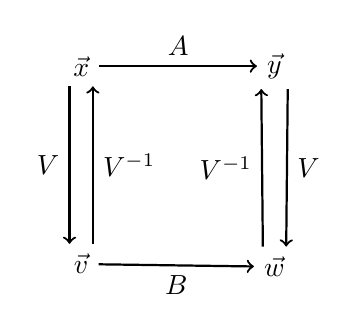
\begin{tikzpicture}[node distance = 2cm, thick]%
        \node (1) {$\vec{x}$};
        \node (2) [right=of 1] {$\vec{y}$};
        \node (3) [below=of 2] {$\vec{w}$};
        \node (4) [below=of 1] {$\vec{v}$};
        \draw[->] (1) -- node [midway,above] {$A$} (2);
        \draw[->] (1.240) -- node [midway,left]{$V$} (4.120);
        \draw[->] (4.60) -- node [midway,right]{$V^{-1}$} (1.300);
        \draw[->] (2.300) -- node [midway,right]{$V$} (3.60);
        \draw[->] (3.120) -- node [midway,left]{$V^{-1}$} (2.240);
        \draw[->] (4) -- node [midway,below] {$B$} (3);
      \end{tikzpicture}%
    \end{figure}
  }
  % % Part(c) solution
  % \sol{
  %   Start by writing $\vec{x_1}$ in terms of $\vec{z_1}$:
  %   $$ \vec{x_1} = V \vec{z_1} $$
  %   Then, apply the transformation $A$ to $\vec{x_1}$, substituting $V \vec{z_1}$ for $\vec{x_1}$:
  %   $$ \vec{x_2} = A V \vec{x_1} $$
  %   Finally, left-multiply both sides by $V^{-1}$ to change $\vec{x_2}$ to the eigenbasis:
  %   $$ \vec{z_2} = V^{-1} \vec{x_2} = V^{-1} A V \vec{z_1} $$

  %   $$A' = V^{-1} A V =
  %   \begin{bmatrix}
  %     1 & 1 \\
  %     -2 & 1
  %   \end{bmatrix}^{-1}
  %   \begin{bmatrix}
  %     3 & -1 \\
  %     -2 & 4
  %   \end{bmatrix}
  %   \begin{bmatrix}
  %     1 & 1 \\
  %     -2 & 1
  %   \end{bmatrix}
  %   $$

  %   $A'$ represents the transformation $A$ in the eigenbasis of $A$, so we know that $A'$ is the diagonal matrix:
  %   $$ A' =
  %   \begin{bmatrix}
  %     \lambda_1 & 0 \\
  %     0 & \lambda_2
  %   \end{bmatrix} =
  %   \begin{bmatrix}
  %     5 & 0 \\
  %     0 & 2
  %   \end{bmatrix} $$

  %   In general, suppose we have a linear transformation $T$ represented by a $n \times n$ matrix that transforms $\vec{u} \in \R^{n}$ to $\vec{v} \in \R^{n}$:
  %   \[
  %     \vec{v} = T\vec{u}
  %   .\]
  %   Suppose we have a basis vectors $\vec{a_1}, \cdots, \vec{a_n} \in \R^{n}$, and the vectors $\vec{u}, \vec{v}$ above are represented in this basis:
  %   \[
  %     \begin{aligned}
  %       \vec{u_a} &= u_{a_1}\vec{a_1} + \cdots + u_{a_n}\vec{a_n} \\
  %       \vec{v_a} &= v_{a_1}\vec{a_1} + \cdots + v_{a_n}\vec{a_n}.
  %     \end{aligned}
  %   \]
  %   Thus we have
  %   \[
  %     \begin{aligned}
  %       T\vec{u}          &= \vec{v} \\
  %       TA\vec{u_a}       &= A\vec{v_a} \\
  %       A^{-1}TA\vec{u_a} &= \vec{v_a}.
  %     \end{aligned}
  %   \]
  %   By pattern matching, we see that if we set $T_a = A^{-1}TA$, we get the relationship $T_a\vec{u_a} = \vec{v_a}$ in the new basis.
  %   The correspondences stated above are all represented in the following diagram:
  %   % \begin{figure}[H]
  %   %   \centering
  %   %   \includegraphics[scale=0.1]{\bank/statespace/figures/change_of_basis.jpg}
  %   % \end{figure}
\end{enumerate}

\newpage
% Author: Yannan Tuo, Varsha Ramakrishnan
% Email: ytuo@berkeley.edu, vio@berkeley.edu
% Edited Lydia Lee, Spring 2019
% lydia.lee@berkeley.edu

\qns{Diagonalization and Other Things Related (ish)}

\begin{enumerate}

\qitem{When is an $n \times n$ matrix diagonalizable, or able to be represented in the form $\mathbf{P}\mathbf{D}^n\mathbf{P}^{-1}$, where $\mathbf{D}$ is a diagonal matrix?}

\meta{An $n\times n$ matrix is diagonalizable when it has $n$ linearly independent eigenvectors, or when the matrix formed by the eigenvectors is full rank. (Note that the eigenvalues do not need to be unique)}


\qitem{Given eigenvalues $\lambda = 1, 2$, diagonalize this matrix 
 $$ \mathbf{A = \begin{bmatrix}
  2 & 0 & 0 \\
  1 & 2 & 1 \\
  -1 & 0 & 1
 \end{bmatrix}}$$
 \\
}

\meta{
[Notice]: A mini lecture may be required before going over the diagonalization problem because students may not have seen this in lecture yet.
For students interested, eigenvalues can be calculated by solving for when $det(A - \lambda I) = 0$ through cofactor expansion (which may not yet taught)
$$det\mathbf{\begin{bmatrix}
  2-\lambda & 0 & 0 \\
  1 & 2-\lambda & 1 \\
  -1 & 0 & 1-\lambda
 \end{bmatrix}}  =  (2 - \lambda)^{2}(1-\lambda)  =  0$$
 $$ \lambda = 1, \lambda = 2 \text{ (2 values)}$$
 }

\sol{

 
Step 1: Find linearly independent eigenvectors of A by solving for the nullspace of $(A-\lambda I)$ for each value of $\lambda$
 $$ \lambda=1 : \mathbf{\begin{bmatrix}
  2-\lambda & 0 & 0 \\
  1 & 2-\lambda & 1 \\
  -1 & 0 & 1-\lambda
 \end{bmatrix}} = 
 \mathbf{\begin{bmatrix}
  1 & 0 & 0 \\
  1 & 1 & 1 \\
  -1 & 0 & 0
 \end{bmatrix}}
 $$
 $$ \hat{v} = \mathbf{\begin{bmatrix}
  0\\
  -1\\
  1
 \end{bmatrix}}
 $$
 
 $$ \lambda=2 : \mathbf{\begin{bmatrix}
  2-\lambda & 0 & 0 \\
  1 & 2-\lambda & 1 \\
  -1 & 0 & 1-\lambda
 \end{bmatrix}} = 
 \mathbf{\begin{bmatrix}
  0 & 0 & 0 \\
  1 & 0 & 1 \\
  -1 & 0 & -1
 \end{bmatrix}}
 $$
 $$ \hat{v} = \mathbf{\begin{bmatrix}
  0\\
  1\\
  0
 \end{bmatrix}}, \mathbf{\begin{bmatrix}
  -1\\
  0\\
  1
 \end{bmatrix}}
 $$
 
 Step 2: Arrange the eigenvectors and eigenvalues into the $\mathbf{P}$ and $\mathbf{D}$ matrices. Note: Make sure to match the row and column of the eigenvalues in the $\mathbf{D}$ matrix with the column of the eigenvectors in the $\mathbf{P}$ matrix.

$$ \mathbf{P = \begin{bmatrix}
  0 & 0 & -1 \\
  -1 & 1 & 0 \\
  1 & 0 & 1
 \end{bmatrix}}
$$
$$
 \mathbf{D = \begin{bmatrix}
  1 & 0 & 0 \\
  0 & 2 & 0 \\
  0 & 0 & 2
 \end{bmatrix}}
 $$
}


\qitem{Consider a pump system with transition matrix $\mathbf{A}$, diagonalized as $\mathbf{P}\mathbf{D}\mathbf{P}^{-1}$. Find the system state $\vec{s}[n]$ given state $\vec{s}[0]$
}

\sol{
\\Use the formula $\vec{s}[n] = \mathbf{A}^n\vec{s}[0]$. We want to calculate $(\mathbf{P}\mathbf{D}\mathbf{P}^{-1})^n\vec{s}[0]$, or 
        $\mathbf{P}\mathbf{D}\mathbf{P}^{-1}\mathbf{P}\mathbf{D}\mathbf{P}^{-1}...\mathbf{P}\mathbf{D}\mathbf{P}^{-1}\vec{s}[0]$. We see that the inner $\mathbf{P}^{-1}$ and $\mathbf{P}$'s cancel out to the identity matrix, leaving us with $\mathbf{P}\mathbf{D}^n\mathbf{P}^{-1}\vec{s}[0]$. 
        \\Consider a sizable matrix $\mathbf{A}$, eg $10 \times 10$, and a large exponent $n$, eg 7. It would generally be computationally simpler to diagonalize the matrix and compute $\mathbf{P}\mathbf{D}^n\mathbf{P}^{-1}\vec{s}[0]$ than to compute $\mathbf{A}^n\vec{s}[0]$ because $\mathbf{D}^n$ involves just raising each number in the diagonal to the $n$th power.
}


\qitem{Is there a relationship between invertibility and diagonizability?
    \begin{enumerate}
        \item  First, let us consider: does invertibility imply diagonizability? Give a brief explanation or counterexample. (Hint: think about how linear independence plays a role in whether or not a matrix is invertible or diagonizable).
    
    \item Does diagonizability imply invertibility? (Hint: think about the invertibility of each individual matrix that constitutes the diagonalized matrix.) %(Note that can't really be used: the determinant of a matrix A is equal to the product of its eigenvalues. If not proven in class, you must prove this yourself.)
    
    \end{enumerate}
}

\sol{
\begin{enumerate}
        \item No, invertibility does not imply diagonalizability. A square matrix is invertible if and only if it has linearly independent columns. For example, take the matrix A and its inverse:
         $$\mathbf{A} =
            \begin{bmatrix}
            2 & 3 \\
            0 & 2 
            \end{bmatrix}, \ \
            \mathbf{A}^{-1} =
            \begin{bmatrix}
            \frac{1}{2} & -\frac{3}{4} \\
            0 & \frac{1}{2}
            \end{bmatrix}$$
        However, when we solve for the eigenvectors, we only get one: $\begin{bmatrix}
            1 \\
            0
            \end{bmatrix}$.
        
        We need two linearly independent vectors to form a diagonalizable matrix; hence, we have found a matrix that is invertible but not diagonalizable. 
        
        Note: remember that one eigenvalue can map to multiple eigenvectors that are linearly independent, so do not confuse the number of eigenvalues with the number of eigenvectors.
        \item False again! Consider the following matrix $M$:
        \begin{align*}
          M &= \begin{bmatrix}1&0\\
                              0&0\end{bmatrix}\\
            &= \begin{bmatrix}1&0\\
                              0&1\end{bmatrix}
                \begin{bmatrix}1&0\\
                               0&0\end{bmatrix}
                \begin{bmatrix}1&0\\
                               0&1\end{bmatrix}
        \end{align*}
        Because $M$ is a diagonal matrix, we can pull its eigenvalues from the diagonal elements to get $\lambda = 0, 1$, and we can compute each eigenspace respectively to get $\vec{v} = \vec{e_2}, \vec{e_1}$ where $\vec{e_i}$ refers to the vector with 1 in its $i$th element and 0 elsewhere.

        However, we also see that the columns (and rows, for that matter) of $M$ are linearly dependent, and so $M$ is not invertible!
\end{enumerate}
}

\end{enumerate}

\newpage
\qns{Mechanical Discretization}

You are building your 16B lab car, and have found the following relation between input voltage and velocity:

\begin{align*}
    \frac{d}{dt} \vec{v}(t) = 5u(t)
\end{align*}
Your MSP can only provide a piecewise constant input voltage with interval $T$. This means that, for each interval $[nT, (n + 1)T)$, $u(t)$ is constant.

\begin{enumerate}
    \qitem You want to analyze your velocity in discrete time as follows:
    \begin{align*}
        v_d(t + 1) = \alpha v_d(t) + u_d(t)
    \end{align*}
    where t is an integer and $v_d(t) = v(tT)$. \\
    \textit{Note: the $t$ in $v_d(t)$ is the current timestep in discrete time (which is always an integer) and differs from the $t$ in $v(t)$, which is in continuous time.}
    \begin{enumerate}[label=(\roman*)]
        \item Find $v(t + T)$ in terms of $v(t)$ and $u(t)$. Say that the input is constant between times $t$ and $t + T$. \\
        \textit{Hint: Integrate both sides and apply the Fundamental Theorem of Calculus.}

        \item Using your result from part (i), find $\alpha$ and $u_d(t)$ in the relation
        \begin{align*}
            v_d(t + 1) = \alpha v_d(t) + u_d(t)
        \end{align*}
    \end{enumerate}

    \qitem Now you want to examine your car's position in discrete time, knowing that
    \begin{align*}
        \frac{d}{dt} x(t) = v(t)
    \end{align*}

    \begin{enumerate}[label=(\roman*)]
        \item Integrate both sides to get $x(t + T)$ in terms of $x(t)$, $v(t)$, and $u(t)$. Again, assume a constant input between times $t$ and $t + T$. \\
        \textit{Hint: If we know $v(t)$, then we can write $v(\tau)$ as $v(t) + v'(t) \cdot (\tau - t)$.}

        \item Discretize the system by finding $\alpha$, $\beta$, and $u_d(t)$ in the following relation
        \begin{align*}
            x_d(t + 1) = \alpha x_d(t) + \beta v_d(t) + u_d(t)
        \end{align*}
    \end{enumerate}

\end{enumerate}
\newpage
% Authors: Taejin Hwang
% Emails: taejin@berkeley.edu

\qns{System Identification}

In this question, we will take a look at how to \textbf{identify} a system by taking experimental data taken from a (presumably) linear system to learn a discrete-time linear model for it using the least-squares.

Recall that a \textbf{linear, continuous-time,} system can be put in state-space form:
\begin{equation}
\ddt{}{t} \vec{x}(t) = A \vec{x}(t) + \vec{b} u(t)
\end{equation}

Now let's say we have an \textbf{unknown} linear system in which we can give an input $u(t)$ and observe the output $\vec{x}(t).$ We can model the system using the following diagram:
\begin{center}
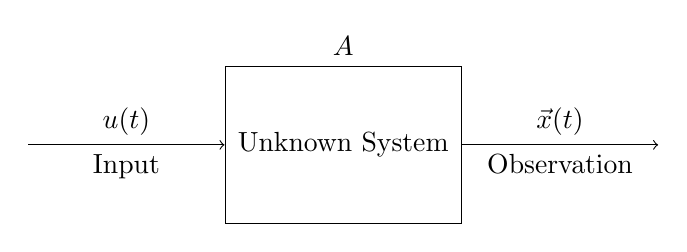
\begin{tikzpicture}
\node[draw, rectangle, minimum width = 3 cm, minimum height = 2 cm] (fl) at (0,0) {Unknown System};
\node[above] at (fl.north) {$A$};
\draw[<-] (fl) -- node[above]{$u(t)$} node[below]{Input} ++(-4,0);
\draw[->] (fl) -- node[above]{$\vec{x}(t)$} node[below]{Observation} ++(4,0);
\end{tikzpicture}
\end{center}

Recall from discussion that if we put a \textbf{piecewise constant} input $u(t) = u[n]$ for $t \in [nT, (n+1)T)$, where $T$ is the interval between samples, then we can observe the output $\vec{x}(t)$ at the $(n+1)^\text{th}$ time step and form a discretized model of the observation.

\begin{center}
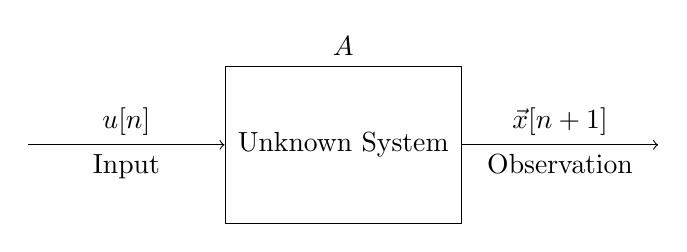
\begin{tikzpicture}
\node[draw, rectangle, minimum width = 3 cm, minimum height = 2 cm] (fl) at (0,0) {Unknown System};
\node[above] at (fl.north) {$A$};
\draw[<-] (fl) -- node[above]{$u[n]$} node[below]{Input} ++(-4,0);
\draw[->] (fl) -- node[above]{$\vec{x}[n + 1]$} node[below]{Observation} ++(4,0);
\end{tikzpicture}
\end{center}

\textbf{If} we knew the system, the relationship for between $\vec{x}[n+1], \ \vec{x}[n], $ and $u[n]$ would be:
\begin{equation}
\vec{x}[n + 1] = A \vec{x}[n] + \vec{b} u[n]
\end{equation}

While this relation is useful, we currently do not know what the $A$ matrix or $\vec{b}$ vector are. \textbf{The goal of system identification is to find $A$ and $\vec{b}$ from data to determine the dynamics of the system.}

For the purposes of this question, our state space will be $\mathbb{R}^2.$ \vskip 1pt
Therefore, we will start by creating unknown variables for the $A$ matrix, and $\vec{b}$ vector:
\begin{equation}
A = \begin{bmatrix} a_{11} & a_{12} \\ a_{21} & a_{22} \end{bmatrix} \ \ \text{and} \ \ \vec{b} = \begin{bmatrix} b_{1} \\ b_{2} \end{bmatrix}
\end{equation}

\begin{enumerate}
  \qitem Let's say the system initially started at $\vec{x}[0] = \begin{bmatrix} x_{1}[0] \\ x_{2}[0] \end{bmatrix},$ and we gave an input at time $t = 0, \ u[0].$ 
  At time $t = 1,$ we observe $\vec{x}(1) = \begin{bmatrix} x_{1}[1] \\ x_{2}[1] \end{bmatrix}.$
  
  \textbf{How can you uncouple this matrix/vector equation into a system of linear equations?}
  Hint: What are the unknowns that you are solving for?

  \ws {
    \vspace{75px}
  }

  \sol {
    We start by writing out the matrix/vector equation for our unknown system:
    \begin{equation}
    \vec{x}(1) = \begin{bmatrix} x_{1}(1) \\ x_{2}(1) \end{bmatrix} = A \vec{x}(0) + \vec{b} u(0) = 
    \begin{bmatrix} a_{11} & a_{12} \\ a_{21} & a_{22} \end{bmatrix} \begin{bmatrix} x_{1}(0) \\ x_{2}(0) \end{bmatrix} + 
    \begin{bmatrix} b_{1} \\ b_{2} \end{bmatrix} u(0)
    \end{equation}

    Uncoupling these equations, we get:
    \pagebreak[0]
    \begin{gather*}
    x_{1}(1) = a_{11} x_{1}(0) + a_{12} x_{2}(0) + b_{1} u(0) \\
    x_{2}(1) = a_{21} x_{1}(0) + a_{22} x_{2}(0) + b_{2} u(0)
    \end{gather*}
  }

  \qitem Based on the system of linear equations created in the previous part, \textbf{how many unknown} variables do we have? Also, if we have a system of linear equations with $n$ unknown variables, at the minimum, \textbf{how many equations} would we need to solve our system?

  \ws {
    \vspace{75px}
  }
  \sol {
    The unknowns in this system of linear equations are: $a_{11}, a_{12}, a_{21}, a_{22}, b_{1}, b_{2}.$ \vskip 1pt
    If we have a system of linear equations with $n$ unknown variables, we will need at least $n$ equations to solve the system. 
  }

  \qitem We now give another input at $t = 1, \ u[1],$ and observe the resulting state after one more time step $\vec{x}[2].$ \vskip 1pt 
  \textbf{How many more equations do we get from this observation? How many more observations will we need to make until we have enough equations?}

  \ws {
      \vspace{50px}
  }
  \sol {
    We can write out a similar observation as the one made in part(a):
    \begin{equation}
    \vec{x}(2) = \begin{bmatrix} x_{1}(2) \\ x_{2}(2) \end{bmatrix} = A \vec{x}(1) + \vec{b} u(1) = 
    \begin{bmatrix} a_{11} & a_{12} \\ a_{21} & a_{22} \end{bmatrix} \begin{bmatrix} x_{1}(1) \\ x_{2}(1) \end{bmatrix} + 
    \begin{bmatrix} b_{1} \\ b_{2} \end{bmatrix} u(1)
    \end{equation}

    Uncoupling these equations again, we will get:
    \pagebreak[0]
    \begin{gather*}
    x_{1}(2) = a_{11} x_{1}(1) + a_{12} x_{2}(1) + b_{1} u(1) \\
    x_{2}(2) = a_{21} x_{1}(1) + a_{22} x_{2}(1) + b_{2} u(1)
    \end{gather*}
    Notice that for every observation we make at a given time step, we will get $2$ more equations. 
    Taking the initial condition $\vec{x}(0)$ into account, we will have to make $4$ observations total, to get $6$ equations.
    In other words, we will have to start observing $\vec{x}(0)$ and continue up until $\vec{x}(3),$ to solve our system.
  }

  \qitem Assume we have collected all of the necessary measurements of $x[n]$ at time $n = 0, 1, 2, \ldots$ by letting the system run its course and recording the state variables at each time step. \vskip 1pt
  \textbf{How can we set up our system of linear equations as a matrix-vector equation?}

  \ws {
    \vspace{75px}
  }
  \sol {
    We can set up the following system of linear equations:
    $$
    \begin{bmatrix}
    x_{1}(0) & x_{2}(0) & u(0) & 0 & 0 & 0 \\
    x_{1}(1) & x_{2}(1) & u(1) & 0 & 0 & 0 \\
    x_{1}(2) & x_{2}(2) & u(2) & 0 & 0 & 0 \\
    0 & 0 & 0 & x_{1}(0) & x_{2}(0) & u(0) \\
    0 & 0 & 0 & x_{1}(1) & x_{2}(1) & u(1) \\
    0 & 0 & 0 & x_{1}(2) & x_{2}(2) & u(2) 
    \end{bmatrix} 
    \begin{bmatrix} a_{11} \\ a_{12} \\ b_{1} \\ a_{21} \\ a_{22} \\ b_{2} \end{bmatrix}
    = \begin{bmatrix} x_{1}(1) \\ x_{1}(2) \\ x_{1}(3) \\ x_{2}(1) \\ x_{2}(2) \\ x_{2}(3) \end{bmatrix}$$
    This can be written in as a matrix vector equation $D \vec{s} = \vec{y}$ and we can solve for $\vec{s} = D^{-1} \vec{y}$  
  }

  \qitem While we can set up a matrix vector equation and uniquely solve our system, the output of the system can be noisy.
  Therefore, we update our model by considering a noise term $w[n]$ at time $t = nT.$
  \begin{equation}
    \vec{x}[n + 1] = A \vec{x}[n] + \vec{b} u[n] + w[n]
  \end{equation}
  \textbf{How can we set up a system of equations in a similar fashion but with a noise vector $\vec{w}$?}

  \begin{equation}
    \vec{y} = D \vec{s} + \vec{w}
  \end{equation}

  \ws {
    \vspace{75px}
  }
  \sol {
    $$
    \begin{bmatrix} x_{1}(1) \\ x_{1}(2) \\ x_{1}(3) \\ x_{2}(1) \\ x_{2}(2) \\ x_{2}(3) \end{bmatrix} 
    = 
    \begin{bmatrix}
    x_{1}(0) & x_{2}(0) & u(0) & 0 & 0 & 0 \\
    x_{1}(1) & x_{2}(1) & u(1) & 0 & 0 & 0 \\
    x_{1}(2) & x_{2}(2) & u(2) & 0 & 0 & 0 \\
    0 & 0 & 0 & x_{1}(0) & x_{2}(0) & u(0) \\
    0 & 0 & 0 & x_{1}(1) & x_{2}(1) & u(1) \\
    0 & 0 & 0 & x_{1}(2) & x_{2}(2) & u(2) 
    \end{bmatrix} 
    \begin{bmatrix} a_{11} \\ a_{12} \\ b_{1} \\ a_{21} \\ a_{22} \\ b_{2} \end{bmatrix}
    + \begin{bmatrix} w(0) \\ w(1) \\ w(2) \\ w(0) \\ w(1) \\ w(2) \end{bmatrix} $$
  }

  \qitem We can try to solve our system of equations, but we do not know what $\vec{w}$ is, so we must assume some small amount of error in our data and solve the for the \textit{best estimate} of the system parameters $A$ and $\vec{b}$. \vskip 1pt
  To do this, we take many measurements (the more data, the better our estimate), and set up a \textbf{least squares} problem as seen in EECS16A.
  \textbf{What would the least squares problem be if we took measurements up to time step $t = 5$?}

  \ws {
    \vspace{100px}
  }
  \sol {
  $$
    \begin{bmatrix} x_{1}(1) \\ x_{1}(2) \\ x_{1}(3) \\ x_{1}(4) \\ x_{1}(5) \\ x_{2}(1) \\ x_{2}(2) \\ x_{2}(3) \\ x_{2}(4) \\ x_{2}(5) \end{bmatrix} 
    = 
    \begin{bmatrix}
    x_{1}(0) & x_{2}(0) & u(0) & 0 & 0 & 0 \\
    x_{1}(1) & x_{2}(1) & u(1) & 0 & 0 & 0 \\
    x_{1}(2) & x_{2}(2) & u(2) & 0 & 0 & 0 \\
    x_{1}(3) & x_{2}(3) & u(3) & 0 & 0 & 0 \\
    x_{1}(4) & x_{2}(3) & u(4) & 0 & 0 & 0 \\
    0 & 0 & 0 & x_{1}(0) & x_{2}(0) & u(0) \\
    0 & 0 & 0 & x_{1}(1) & x_{2}(1) & u(1) \\
    0 & 0 & 0 & x_{1}(2) & x_{2}(2) & u(2) \\
    0 & 0 & 0 & x_{1}(3) & x_{2}(3) & u(3) \\
    0 & 0 & 0 & x_{1}(4) & x_{2}(4) & u(4) 
    \end{bmatrix} 
    \begin{bmatrix} a_{11} \\ a_{12} \\ b_{1} \\ a_{21} \\ a_{22} \\ b_{2} \end{bmatrix}
    + \begin{bmatrix} w(0) \\ w(1) \\ w(2) \\ w(3) \\ w(4) \\ w(0) \\ w(1) \\ w(2) \\ w(3) \\ w(4) \end{bmatrix} $$

    Which can equivalently be written as:
    \begin{equation}
      \vec{y} = D \vec{s} + \vec{w}
    \end{equation}
    For the least squares problem, we will want to minimize $\norm{\vec{w}}_{2} = \norm{y - D \vec{s}}_{2}$
    }

  \qitem \textbf{How would we solve this least squares problem? What conditions need to be satisfied in our data for the least squares problem to have a unique solution?}

  \ws {
    \vspace{75px}
  }
  \meta {
    You can show that $D$ and $D^{T}D$ have the same null spaces, to claim that if $D$ is full rank, then $D^{T}D$ will be invertible.
  }

  \sol {
    Recall from 16A that if we are given the least squares problem:
    \begin{equation}
      A \vec{x} = \vec{b} + \vec{e}
    \end{equation}
    The solution that minimizes the norm of the residual $\norm{\vec{e}}_{2}$ is:
    \begin{equation}
      \vec{\hat{x}} = (A^{T} A)^{-1} A^{T} \vec{b}
    \end{equation}
    Therefore the solution to the least squares problem above will be:
    \begin{equation}
      \vec{\hat{s}} = (D^{T} D)^{-1} D^{T} \vec{y}
    \end{equation}
    The $\vec{\hat{s}}$ will give the best possible estimate for the $A$ and $\vec{b}.$ \vskip 1pt
    A concern we shoud make is whether or not $D^{T} D$ is an invertible matrix.
    Remember that is $D$ is full rank, then $D^{T} D$ will be invertible.
  }
\end{enumerate}


\newpage


\end{qunlist}

\end{document}
